\documentclass[border=2mm]{standalone}

\usepackage[dvipsnames]{xcolor}
\usepackage{tikz}
\usetikzlibrary{positioning, arrows, shadows.blur}

\begin{document}

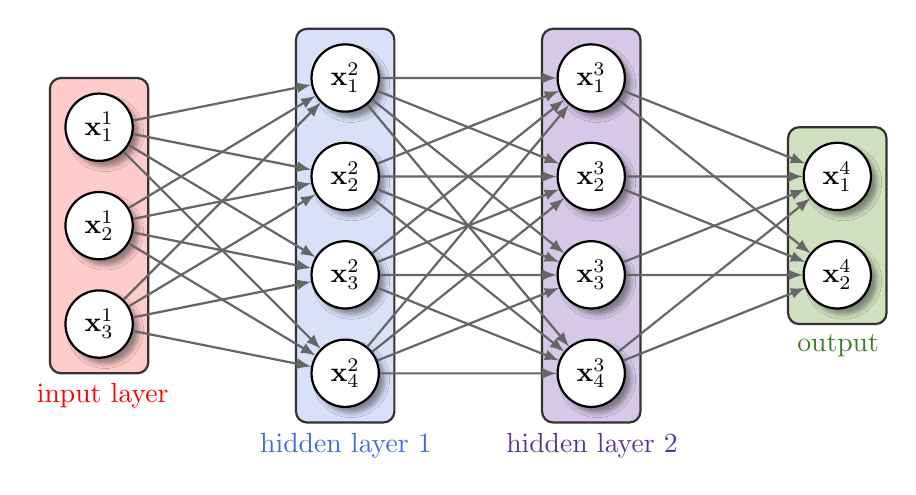
\begin{tikzpicture}[
  neuron/.style = {
    circle,
    draw,
    thick,
    fill = white,
    blur shadow
  },
  connection/.style = {
    -latex,
    black!60,
    thick
  },
  box/.style = {
    draw = black!80,
    thick,
    rounded corners
  },
  scale = 1.25,
  ]
  % \draw[help lines, red] (-1, 0) grid (8, -5);

  % Bounding box input layer.
  \draw[box, fill=red!20] (-.5, -1) rectangle (.5, -4)
  node[below, red, xshift=-16.5] {input layer};
  % Bounding box first hidden layer.
  \draw[box, fill=RoyalBlue!20] (2, -.5) rectangle (3, -4.5)
  node[below, RoyalBlue, xshift=-17.5] {hidden layer 1};
  % Bounding box second hidden layer.
  \draw[box, fill=RoyalPurple!20] (4.5, -.5) rectangle (5.5, -4.5)
  node[below, RoyalPurple, xshift=-17.5] {hidden layer 2};
  % Bounding box output layer.
  \draw[box, fill=OliveGreen!20] (7, -1.5) rectangle (8, -3.5)
  node[below, OliveGreen, xshift=-17.5] {output};

  % Neurons input layer.
  \begin{scope}[shift={(0, -.5)}]
    \foreach \name in {1,...,3} {
      \node[neuron] (I-\name) at (0, -\name) {$\mathbf{x}_\name^{1}$};
    }
  \end{scope}
  % Neurons first hidden layer.
  \foreach \name in {1,...,4} {
    \node[neuron] (H1-\name) at (2.5, -\name) {$\mathbf{x}_\name^{2}$};
  }
  % Neurons second hidden layer.
  \foreach \name in {1,...,4} {
    \node[neuron] (H2-\name) at (5, -\name) {$\mathbf{x}_\name^{3}$};
  }
  % Node output layer.
  \begin{scope}[shift={(0, -1)}]
    \foreach \name in {1,...,2} {
      \node[neuron] (O-\name) at (7.5, -\name) {$\mathbf{x}_\name^{4}$};
    }
  \end{scope}

  % Connections between input and first hidden layers.
  \foreach \source in {1,...,3} {
    \foreach \dest in {1,...,4} {
      \path[connection] (I-\source) edge (H1-\dest);
    }
  }
  % Connections between first and second hidden layers.
  \foreach \source in {1,...,4} {
    \foreach \dest in {1,...,4} {
      \path[connection] (H1-\source) edge (H2-\dest);
    }
  }
  % Connection between second hidden layer and output.
  \foreach \source in {1,...,4} {
    \foreach \dest in {1,...,2} {
      \path[connection] (H2-\source) edge (O-\dest);
    }
  }
\end{tikzpicture}

\end{document}